
\newpage

\section{Resultados e Análise de Dados}

\subsection{FPB}
O primeiro filtro projetado foi um filtro passa-baixas de terceira ordem, com 
resposta do tipo Butterworth utilizando apenas 1 indutor.



A figura \ref{fFPB} mostra o circuito utilizado.\begin{figure}[H]
  \centering
  
  %    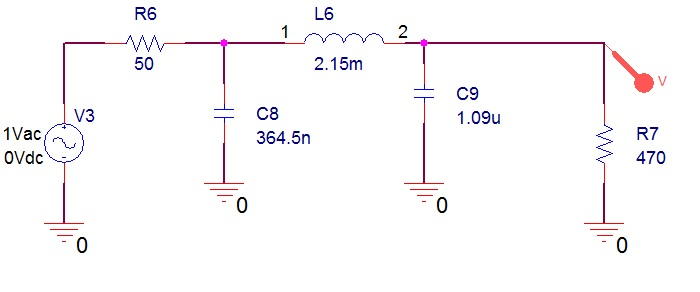
\includegraphics[scale=0.8]{Imagens/fpb.jpg}
  \label{fFPB}
  \caption{Filtro desnormalizado passa-baixas.}
\end{figure}



\subsection{FPA}
O segundo filtro projetado foi um filtro passa-altas de terceira ordem, com 
resposta do tipo Butterworth utilizando apenas 1 indutor. A frequência de corte 
dada é de 4,2 kHz, o resistor da fonte $R_s = 470 \Omega$ e a carga $R_l = 50 
\Omega$.

Foram analisadas a frequência de corte, atenuação fora da faixa de passagem, 
atenuação na faixa de passagem e a defasagem ao longo de toda a faixa de 
frequências.

A figura \ref{fFPA} mostra o circuito utilizado.\begin{figure}[H]
  \centering
  % 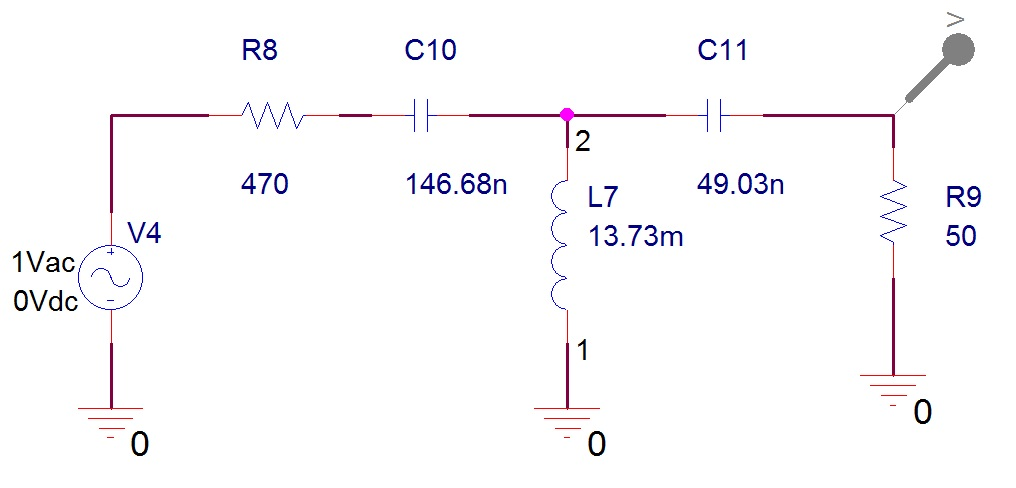
\includegraphics[scale=0.5]{Imagens/fpa.jpg}
  \label{fFPA}
  \caption{Filtro desnormalizado passa-altas.}
\end{figure}

\subsection{FPF em cascata}
No terceiro circuito o filtro FPB e o FPA desenvolvidos anteriormente foram 
conectados em cascata de forma a formar um filtro passa-faixa, onde foi também 
analisado a largura de banda passante do filtro.

Na figura \ref{fFPFC} é apresentado o circuito resultante da conexão dos filtro 
FPA e FPB, na topologia cascata.

\begin{figure}[H]
  \centering
  % 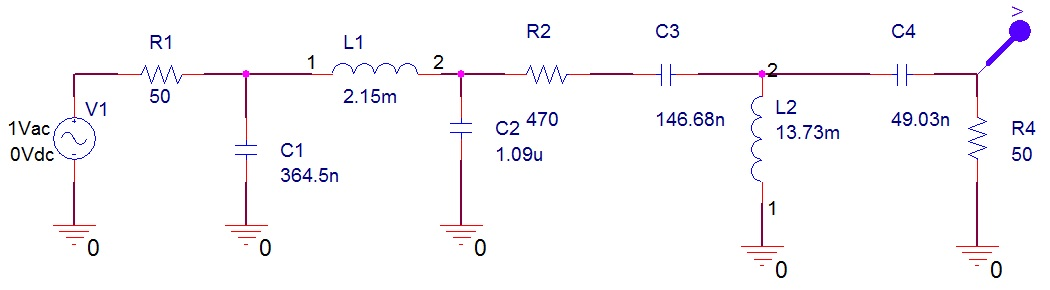
\includegraphics[scale=0.5]{Imagens/fpf1.jpg}
  \label{fFPFC}
  \caption{Filtro passa-faixa em cascata.}
\end{figure}

\subsection{FPF}
O quarto e ultimo filtro foi projetado para ter uma resposta em frequência 
semelhante a do filtro FPF em cascata. O objetivo foi de analisar as diferenças 
em se utilizar um filtro FPF e um filtro FPB em conjunto com um filtro FPA.

A figura \ref{fFPF} representa o filtro passa-faixa projetado.

\begin{figure}[H]
  \centering
  % 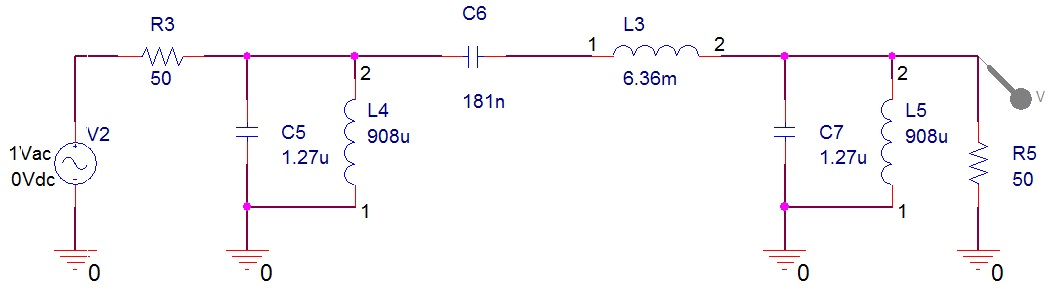
\includegraphics[scale=0.5]{Imagens/fpf2.jpg}
  \label{fFPF}
  \caption{Filtro passa-faixa.}
\end{figure}